\documentclass[11pt]{article}
\usepackage[letterpaper,margin=0.9in]{geometry}
\usepackage[T1]{fontenc}
\usepackage{lmodern}
\usepackage{microtype}
\usepackage{xcolor}
\usepackage{graphicx}
\usepackage{array,tabularx,booktabs}
\usepackage{enumitem}
\usepackage{caption}
\usepackage{amssymb}
\usepackage[hidelinks]{hyperref}

\setlength{\parindent}{0pt}
\setlength{\parskip}{5pt}
\setlist[itemize]{leftmargin=1.3em,topsep=2pt,itemsep=2pt,parsep=0pt}
\setlist[enumerate]{leftmargin=1.5em,topsep=2pt,itemsep=2pt,parsep=0pt}
\captionsetup{font=small,labelfont=bf,skip=4pt}
\newcolumntype{Y}{>{\raggedright\arraybackslash}X}
\definecolor{boxbg}{HTML}{F6F1EC}
\definecolor{donec}{HTML}{2E7D32}
\definecolor{todoc}{HTML}{C2571A}
\newcommand{\keybox}[1]{\par\smallskip\noindent\colorbox{boxbg}{\parbox{\dimexpr\linewidth-2\fboxsep}{\vspace{3pt}#1\vspace{3pt}}}\par\smallskip}
\newcommand{\done}{\textcolor{donec}{\checkmark}}
\newcommand{\todo}{\textcolor{todoc}{$\square$}}

\title{\textbf{Benchmark Cartography}\\[2pt]
\large The whole project explained: what it is, what is done, and what we do next}
\author{Team 21: Arman Samayam and Padmapriya Venkatesh\\
\small DS-GA 3001 Visualization for Machine Learning, NYU, Fall 2026 $\cdot$ Status as of November 27, 2026}
\date{}

\begin{document}
\maketitle
\vspace{-2em}

\keybox{\textbf{In one sentence.} By having 150 AI models ``vote'' on every question of a famous AI
exam, we spot questions whose official answer is probably wrong, often suggest the right one, and
show in an interactive tool that these mistakes reshuffle the middle of the AI leaderboard, though
not the top. Because the models can all be wrong together, a person still makes the final call.

\smallskip
\textbf{Where we are.} The data, analysis, tool and report are built, and the checks between the two
of us are done. Because we could not recruit experts over Thanksgiving week, we present three
\emph{usage scenarios} on December 1, then run 2--3 short expert sessions with the course TAs before
the final report. What remains: the final report edits, the presentation, and those sessions.}

\section*{Part 1. The project}

\section{The problem}

AI language models (like the one behind ChatGPT) are compared by giving them the same exam, called a
\textbf{benchmark}. One of the most used is \textbf{MMLU}: about \textbf{14,000 multiple-choice
questions} (A--D) in \textbf{57 subjects}, each with an official \textbf{answer key}. Public
\textbf{leaderboards} rank hundreds of models by their percentage correct.

The answer key has mistakes. Experts from the \textbf{MMLU-Redux} project hand-checked 5,700 questions
and found about \textbf{2\% with a wrong key} and 4--5\% more that are unclear or have no single right
answer. A model that picks the truly correct answer to a mis-keyed question is marked wrong. About
\textbf{8,300 questions have never been checked}, and neighbouring models on the leaderboard are often
less than a fifth of a percentage point apart.

We ask: (1) can we \textbf{find} the broken questions automatically, and (2) does fixing them
\textbf{change the leaderboard}?

\section{The idea: many models vote}

A public archive (the Open LLM Leaderboard) stores how hundreds of models answered every MMLU
question. We use \textbf{150 models}, all tested the same way.
\begin{itemize}
  \item \textbf{Hard but fair question:} weak models get it wrong, strong models get it right.
  \item \textbf{Wrong key:} even the \textbf{strongest} models get it ``wrong'', and they \textbf{all
    pick the same other answer}, which is usually the real one.
\end{itemize}
The idea adapts \textbf{Dataset Cartography}, which finds mislabelled data by watching one model learn
over time; we watch many models at once instead.

\section{What we measure}

For each question we compute simple scores from the models' probabilities: \textbf{confidence} (how
much models believe the official answer), \textbf{variability} (how much they disagree),
\textbf{top-tier confidence} (confidence among the 30 strongest models, our best signal), the
\textbf{consensus alternative} (the answer the strongest models prefer instead, which suggests a fix)
and its \textbf{share}, and \textbf{ability alignment} (do stronger models do better on it?).

Our main comparison is \textbf{Item Response Theory (IRT)}, the standard exam-design method, which
gives each question a difficulty and a discrimination. Our instructor asked us to show what our
approach adds beyond IRT.

\section{The tool}

A website built with D3: \url{https://armansam17.github.io/Benchmark-Cartography/}

\begin{figure}[!htb]
  \centering
  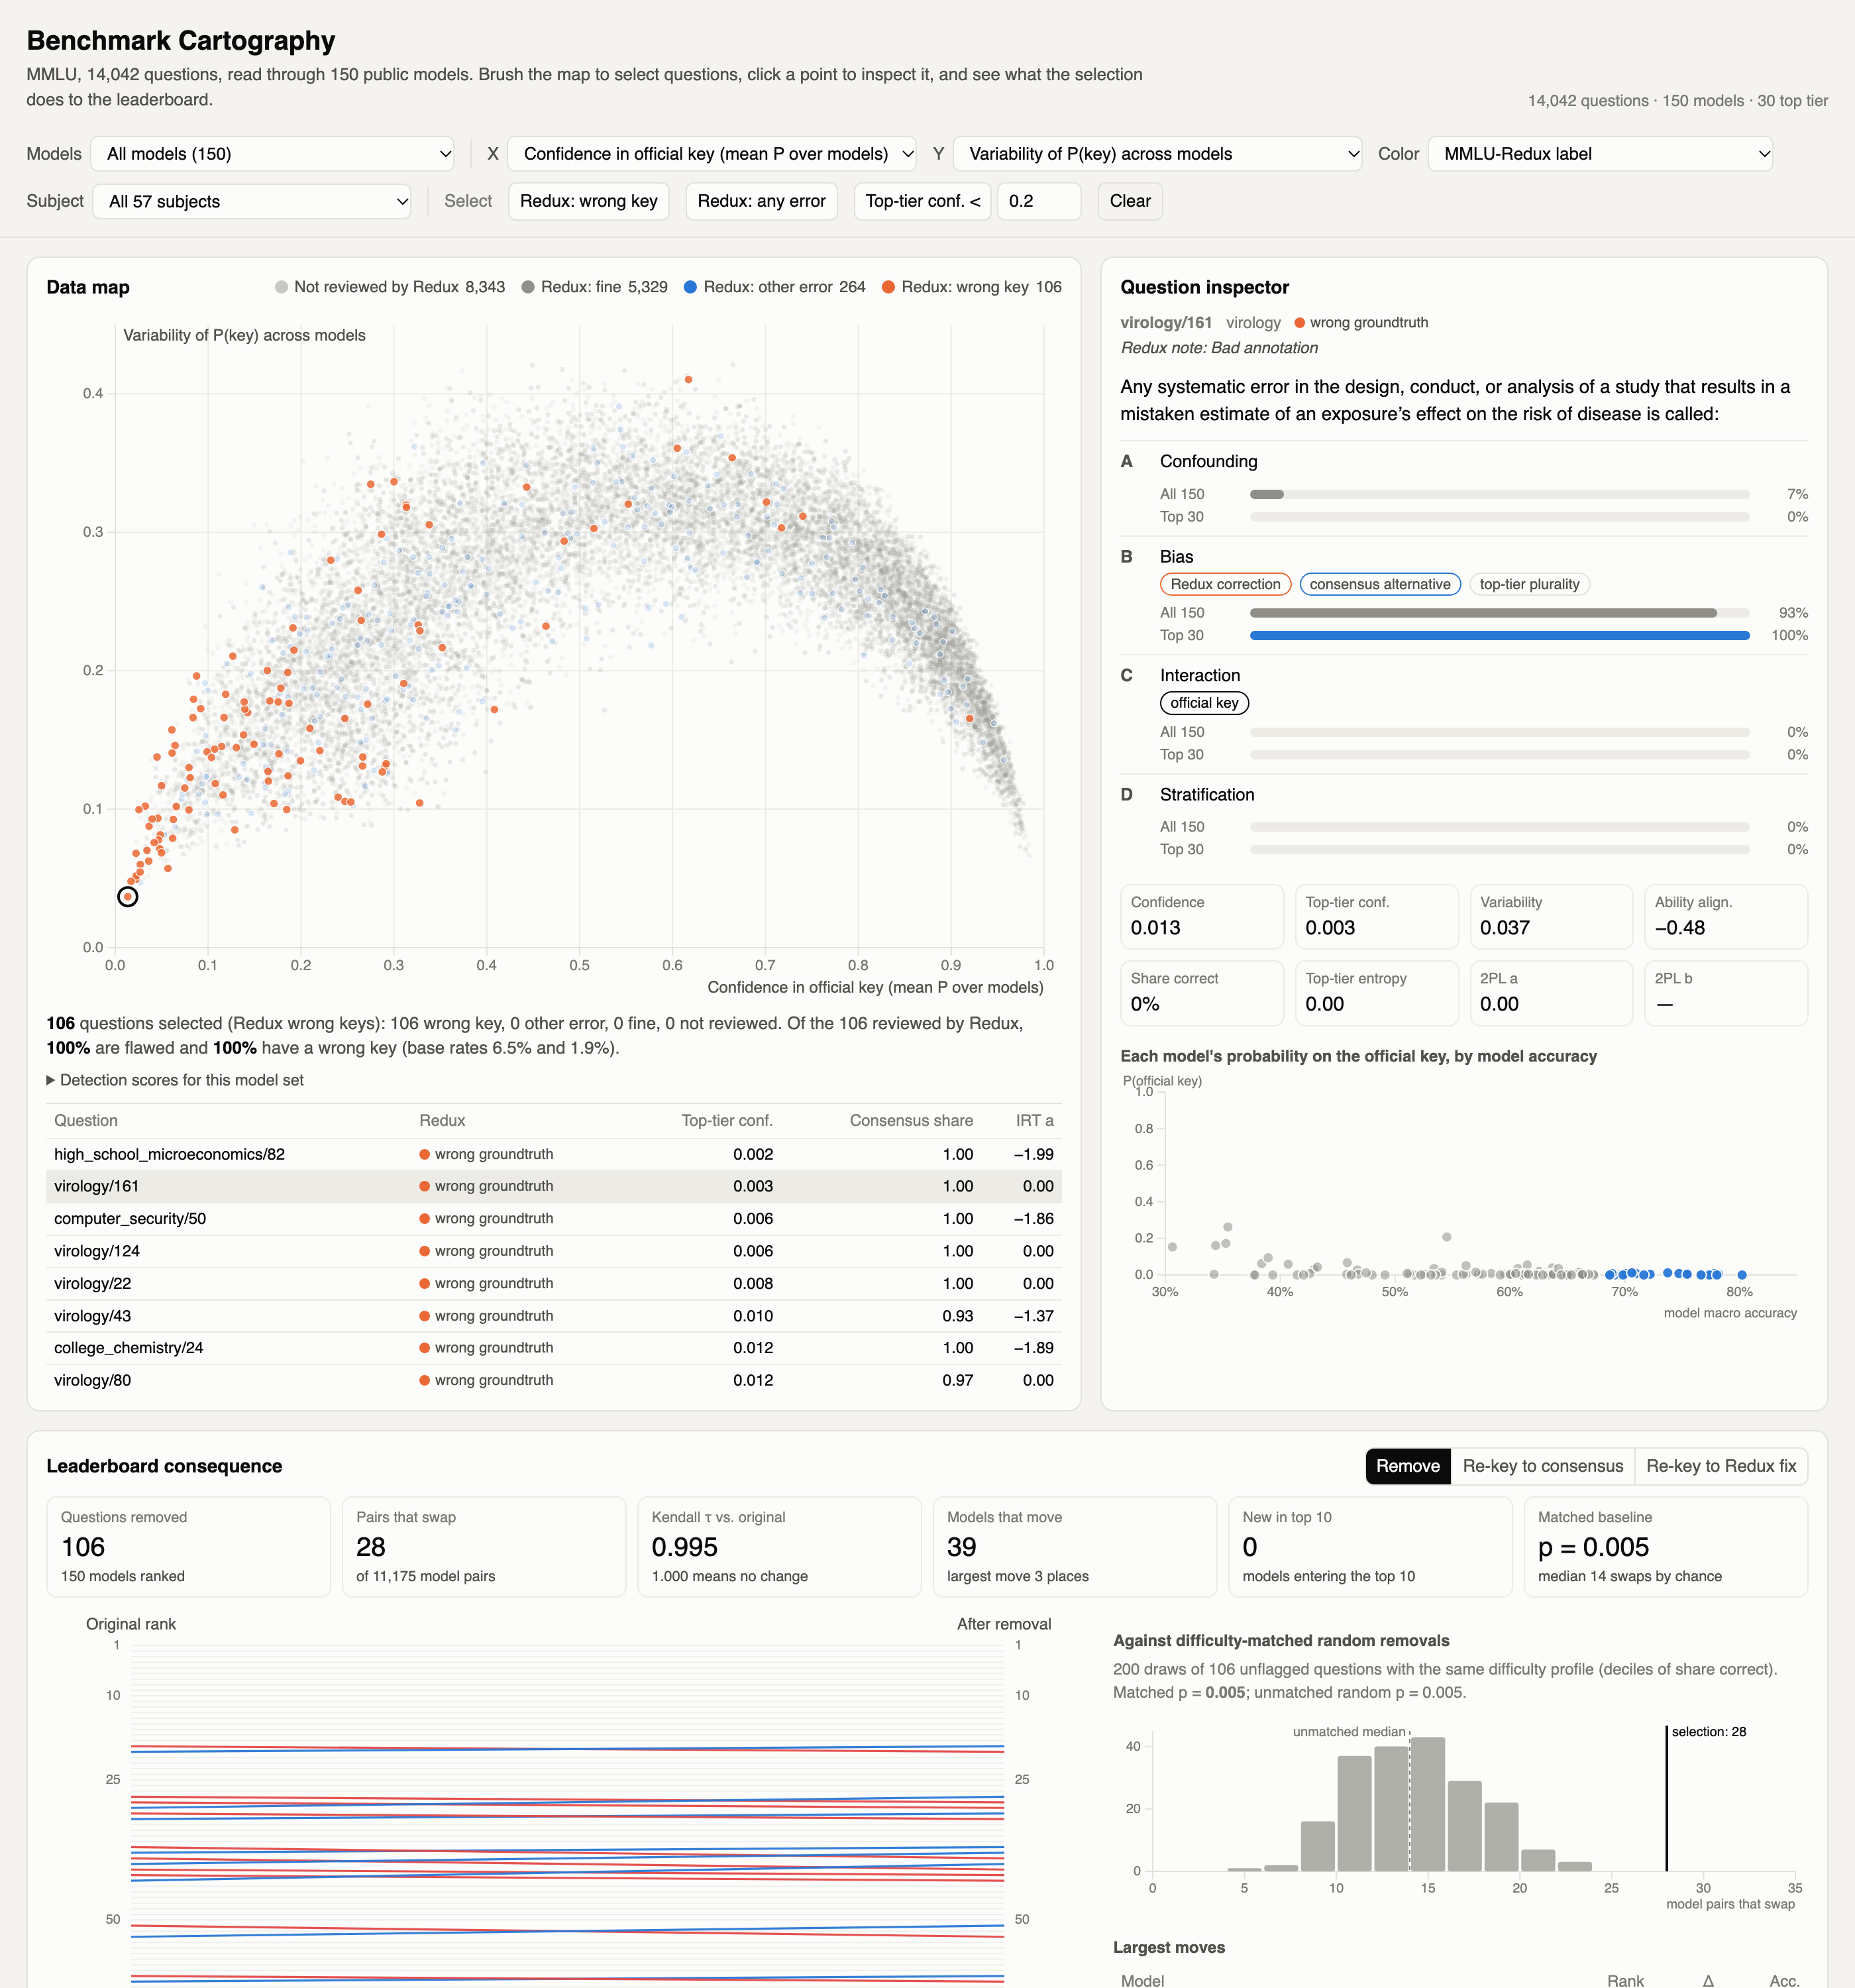
\includegraphics[width=0.92\linewidth]{../report/fig_tool.png}
  \caption{The tool with the 106 known wrong keys selected (orange): the data map (left), the
  question inspector (right) and the leaderboard view (bottom).}
\end{figure}

\begin{itemize}
  \item \textbf{Data map} (``where should I look?''): every question is a dot; wrong keys cluster in
    one corner. Drag a box to select a region.
  \item \textbf{Question inspector} (``is it really broken?''): the question, the key, the answer the
    top models prefer, vote bars for all models and the top 30, and a plot of each model's belief in
    the key against how strong the model is.
  \item \textbf{Leaderboard view} (``does it matter?''): remove or correct the selected questions,
    re-rank all 150 models, and compare against random questions of the same difficulty (a p-value).
  \item \textbf{Extras}: recompute everything on model subsets; a study mode that hides the expert labels.
\end{itemize}

\section{Results}

\begin{enumerate}
  \item \textbf{Wrong keys sit in their own corner.} Top models put a typical 12\% belief on a wrong
    key against 82\% on a normal question. Unclear questions do not form a group.
  \item \textbf{Detection beats IRT, modestly.} On the AUPRC measure (random = 0.019), majority vote
    scores 0.176, IRT difficulty 0.211, and our top-tier confidence \textbf{0.355}. 19 of our 25 most
    suspicious questions are real wrong keys, and when the top models agree on an alternative it
    matches the experts' correction \textbf{87\%} of the time. Our scores overlap heavily with IRT; our
    advantage is what the tool lets a person see next. No method here finds ambiguous questions.
  \item \textbf{The leaderboard changes, but only in the middle.} Removing the 106 known wrong keys
    swaps \textbf{28} model pairs against about 14 for random questions ($p = 0.001$); correcting them
    swaps 50. No model enters or leaves the top 10. Mistakes don't change who is best, but can flip
    comparisons between near-identical models.
  \item \textbf{New suspected errors.} 289 unchecked questions look strongly suspicious, for example
    the \emph{Star Trek II} Vulcan (key: Helen Hunt; top models: Kirstie Alley) and ``which is
    \emph{not} a primary facial expression'' (key: surprise; top models: love). We hand-checked the 20
    most suspicious: 17 have a wrong key, 1 is ambiguous and 2 need the source text to judge.
\end{enumerate}

\section*{Part 2. What changed: usage scenarios instead of an expert study}

\section{Why we changed the evaluation}

Our plan was a \textbf{qualitative think-aloud study}: 3 people who work on AI evaluation would use
the tool while talking through their reasoning, triaging 8 prepared questions. The protocol, the
question set and the tool's study mode are all ready (\texttt{study/}). But it is Thanksgiving week
and we could not get participants to reply in time.

So we replaced it with \textbf{usage scenarios}, a standard way to evaluate visualization tools: we
walk through real tasks in the deployed tool, step by step, with real questions and numbers anyone can
reproduce. We are honest in the report that this shows what the tool \emph{makes possible}, not how
well other people use it.

\textbf{Revised plan.} Usage scenarios carry the December 1 presentation. After it, when people are
back from the break, we run 2--3 short expert sessions (about 20 minutes each) with the course TAs,
using the protocol and study mode that are already built, and add their feedback to the final report
due December 14.

\section{The three scenarios}

\begin{figure}[!htb]
  \centering
  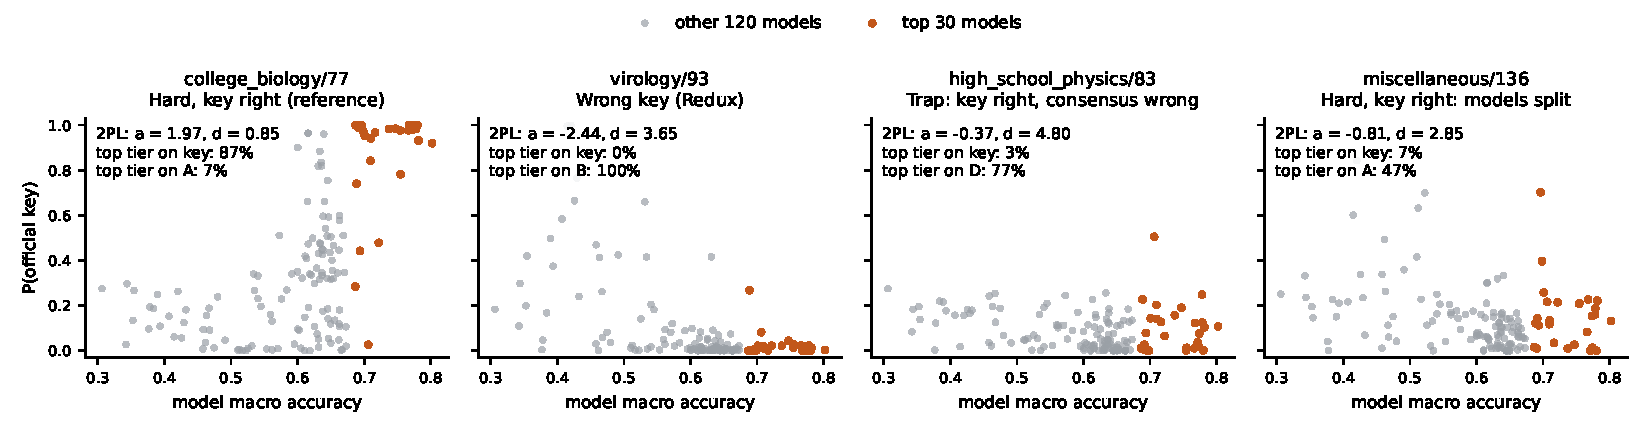
\includegraphics[width=\linewidth]{../report/fig_scenarios.pdf}
  \caption{Each model's belief in the official answer (up) against its overall strength (right); the
  30 strongest models are orange. Left: a fair hard question. The other three look identical to IRT
  but differ in how the models vote.}
\end{figure}

\begin{enumerate}
  \item \textbf{Finding errors nobody checked.} Brush the suspicious corner among the unchecked (grey)
    questions and click through: within minutes the Star Trek and facial-expression questions appear,
    each with a proposed correction.
  \item \textbf{Wrong key, or just hard?} Three questions look identical to IRT, yet the tool tells
    them apart:
    \begin{itemize}
      \item \emph{Filovirus shape:} all 30 top models pick the same alternative: a \textbf{wrong key}.
      \item \emph{``If Christmas is a Saturday, what day is New Year's?''}: the top models split almost
        evenly between two wrong answers: a \textbf{hard question}, and the key is right.
      \item \emph{Concave mirror:} 77\% of top models agree, but \textbf{they are wrong}. Agreement is
        evidence, not proof, so the tool leaves the final call to a person.
    \end{itemize}
  \item \textbf{Does it matter?} Remove the known wrong keys: the ranking reshuffles more than chance,
    but only mid-table, and the effect shrinks but persists on model subsets.
\end{enumerate}

These scenarios also answer the instructor's question about IRT: a table sorted by IRT finds the same
questions, but it cannot show whether models agree or split, what answer they propose, or the
effect on the ranking.

\section*{Part 3. Status and plan}

\section{What is done}

\begin{center}\small
\begin{tabularx}{\linewidth}{@{}p{0.4cm}p{3.4cm}Y@{}}
\toprule
& \textbf{Piece} & \textbf{State} \\
\midrule
\done & Data (Stage 1) & 150 models $\times$ 14,042 questions, joined with MMLU-Redux; scores and
IRT computed; cached with checksums \\
\done & Analysis (Stage 2) & Arman's detection and ranking scripts run and agree with the tool \\
\done & Tool (Stage 3) & Live on GitHub Pages and redeploys automatically on every push; all three
core views, model subsets and study mode work \\
\done & Study materials & Protocol, facilitator key, 8-question study set, session log files \\
\done & Report draft & 8 pages plus references; Section 6 rewritten as usage scenarios with a new
figure; abstract, research question 4, discussion, limitations and conclusion updated \\
\done & Explainers & A beginner's explainer and this status document (\texttt{docs/}) \\
\done & Top-20 hand-check & The 20 most suspicious unreviewed questions: 17 wrong keys, 1 ambiguous,
2 need the source (\texttt{results/handcheck\_top20.csv}) \\
\done & Report checks & Star Trek and facial-expression keys confirmed wrong; ``21 vs.\ 35 swaps''
reading confirmed; p-value formula in \texttt{analysis/02\_ranking.py} matches the tool and report \\
\bottomrule
\end{tabularx}
\end{center}

\section{What we do now}

The checks between us are done. The plan from here, in order:

\begin{center}\small
\begin{tabularx}{\linewidth}{@{}p{0.4cm}Yp{2.4cm}p{2.3cm}@{}}
\toprule
& \textbf{Task} & \textbf{Who} & \textbf{When} \\
\midrule
\todo & Report: add the top-20 result, remove the ``pending confirmation'' and ``confirm this
interpretation'' notes, and drop the HELM sentence & Padmapriya & Nov 28 \\
\todo & Note to the TAs: the live study before Dec 1 became usage scenarios; ask whether each can
give a 20-minute session in the week of Dec 2 & Padmapriya & Nov 28 \\
\todo & Fill or delete every remaining placeholder, recompile, proofread, push & Padmapriya & Nov 28 \\
\todo & Slides (about 10) and a 3-minute live demo: map $\rightarrow$ virology question
$\rightarrow$ mirror trap $\rightarrow$ leaderboard & Both & by Nov 30 \\
\todo & Rehearse the presentation, with a recorded demo as backup & Both & Nov 30 \\
\todo & Present & Both & Dec 1 \\
\todo & Run 2--3 expert sessions (study mode, \texttt{study/expert\_study\_protocol.md}); one
facilitates, one takes notes & Both & Dec 2--10 \\
\todo & Add an expert-feedback subsection to the report; final proofread and submit & Both & by Dec 14 \\
\bottomrule
\end{tabularx}
\end{center}

\textbf{Course dates.} Presentation December 1; final report December 14.

\section{Deliverables at the end}
\begin{itemize}
  \item \textbf{Live tool:} \url{https://armansam17.github.io/Benchmark-Cartography/}
  \item \textbf{Report:} \texttt{report/report.pdf} (8 pages plus references)
  \item \textbf{Code and data:} \url{https://github.com/ArmanSam17/Benchmark-Cartography}; scripts
    regenerate every number and figure
  \item \textbf{Presentation} with a live demo
\end{itemize}

\end{document}
